% !TeX spellcheck = cs_CZ
{\tikzset{external/prefix={tikz/FYZI/}}
 \tikzset{external/figure name/.add={ch38_}{}}
%=========================== Kapitola: Souvislost mezi vlnovým a korpuskulárním hlediskem =========
\chapter{Souvislost mezi vlnovým a korpuskulárním hlediskem}\label{fyz:IchapXXXVIII}
\minitoc
\section{Amplitudy vln pravděpodobnosti}\label{fyz:IchapXXXVIIIsecI}
\section{Měření polohy a hybnosti}\label{fyz:IchapXXXVIIIsecII}
\section{Difrakce na krystalech}\label{fyz:IchapXXXVIIIsecIII}
\section{Velikost atomu}\label{fyz:IchapXXXVIIIsecIV}
\section{Energetické hladiny}\label{fyz:IchapXXXVIIIsecV}
\section{Filozofické důsledky}\label{fyz:IchapXXXVIIIsecVI}
\section{Příklady a cvičení}\label{fyz:IchapXXXVIIIsecVII}

  \begin{figure}[ht!] %\ref{fyz:fig432}
    \centering
    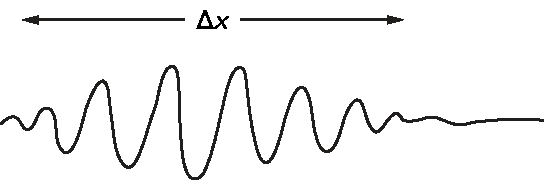
\includegraphics[width=0.7\linewidth]{fyz_fig432.pdf}
    \caption{Vlnový balík délky \(\Delta x\)
             (\cite[s.~510]{Feynman01})}
    \label{fyz:fig432}
  \end{figure}

  \begin{figure}[ht!] %\ref{fyz:fig433}
    \centering
    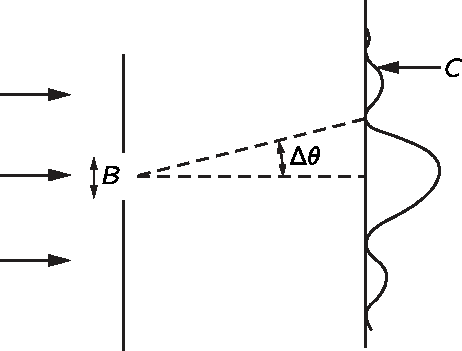
\includegraphics[width=0.7\linewidth]{fyz_fig433.pdf}
    \caption{Difrakce částic procházejících štěrbinou 
             (\cite[s.~511]{Feynman01})}
    \label{fyz:fig433}
  \end{figure}

  \begin{figure}[ht!] %\ref{fyz:fig434}
    \centering
    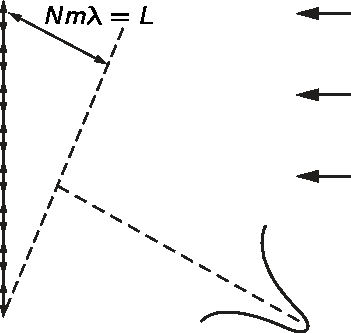
\includegraphics[width=0.7\linewidth]{fyz_fig434.pdf}
    \caption{Určení hybnosti pomocí difrakční mřížky
             (\cite[s.~513]{Feynman01})}
    \label{fyz:fig434}
  \end{figure}

  \begin{figure}[ht!] %\ref{fyz:fig435}
    \centering
    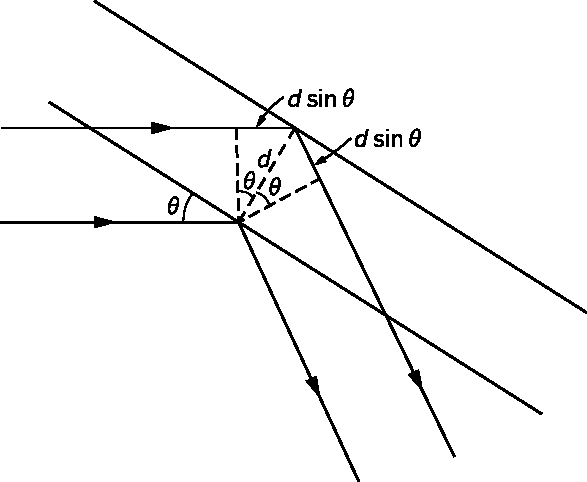
\includegraphics[width=0.7\linewidth]{fyz_fig435.pdf}
    \caption{Rozptyl vln na krystalových rovinách
             (\cite[s.~514]{Feynman01})}
    \label{fyz:fig435}
  \end{figure}

  \begin{figure}[ht!] %\ref{fyz:fig436}
    \centering
    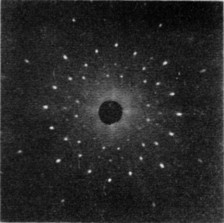
\includegraphics[width=0.7\linewidth]{fyz_fig436.jpg}
    \caption{
             (\cite[s.~515]{Feynman01})}
    \label{fyz:fig436}
  \end{figure}

  \begin{figure}[ht!] %\ref{fyz:fig437}
    \centering
    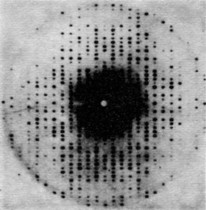
\includegraphics[width=0.7\linewidth]{fyz_fig437.jpg}
    \caption{
             (\cite[s.~515]{Feynman01})}
    \label{fyz:fig437}
  \end{figure}

  \begin{figure}[ht!] %\ref{fyz:fig438}
    \centering
    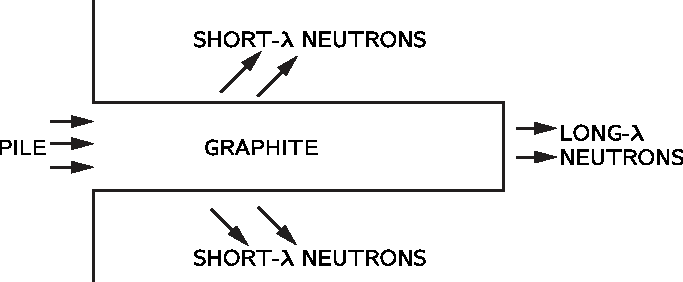
\includegraphics[width=0.7\linewidth]{fyz_fig438.pdf}
    \caption{
             (\cite[s.~515]{Feynman01})}
    \label{fyz:fig438}
  \end{figure}

  \begin{figure}[ht!] %\ref{fyz:fig439}
    \centering
    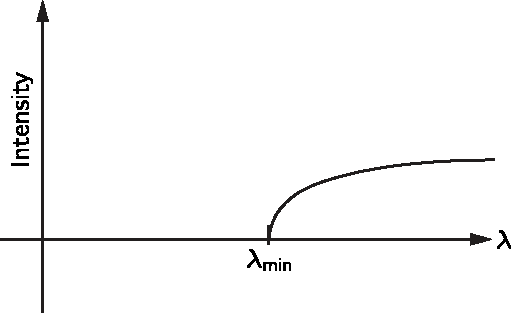
\includegraphics[width=0.7\linewidth]{fyz_fig439.pdf}
    \caption{Intenzita neutronů vyletujících z grafitového bloku jako funkce vlnové délky
             (\cite[s.~516]{Feynman01})}
    \label{fyz:fig439}
  \end{figure}

  \begin{figure}[ht!] %\ref{fyz:fig440}
    \centering
    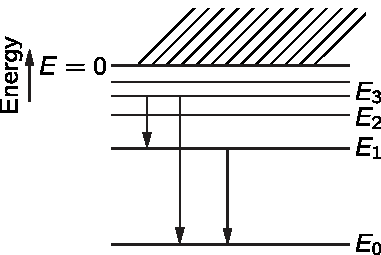
\includegraphics[width=0.7\linewidth]{fyz_fig440.pdf}
    \caption{Energetické schéma atomu znázorňující několik možných přechodů
             (\cite[s.~518]{Feynman01})}
    \label{fyz:fig440}
  \end{figure}
  
} %tikzset
%~~~~~~~~~~~~~~~~~~~~~~~~~~~~~~~~~~~~~~~~~~~~~~~~~~~~~~~~~~~~~~~~~~~~~~~~~~~~~~~~~~~~~~~~~~~~~~~~~~
\printbibliography[title={Seznam literatury}, heading=subbibliography]
\addcontentsline{toc}{section}{Seznam literatury}